\textcolor{lila}{Innan vi började med projektet hade vi uppfattningen att problemlösning, trots den ändrade kursplanen, ändå inte inkluderas tillräckligt mycket i matematikundervisningen på gymnasiet. För att undersöka detta gjordes dels en enkät, och dels genomfördes en längre intervju med en lärare.} 

\subsection{Enkät till matematiklärare om deras undervisning}
\label{sec:Bakgrundsenkat}
\textcolor{lila}{Enkäten skickades ut via en facebook-sida för matematiklärare. Den gav lärarna en chans att berätta till vilken grad och på vilket sätt de arbetar med problemlösning, samt vilka faktorer de anser hindrar dem i detta arbete. Totalt fick vi in 58 svar från lärare över hela Sverige.}

\textcolor{lila}{Resultatet består till största del av fritext där lärarna själva har fått uttrycka sin syn på de olika frågorna. Dessa svar har analyserats och sorterats utifrån olika gemensamma nämnare. De svar som presenteras i kursiv text nedan är alltså inte nödvändigtvis svar från enkäten, men representerar det som vi tolkat som den bakomliggande tanken i de olika svaren. Notera även att ett enskilt svar från en lärare kan falla under flera av dessa kategorier.}

\subsubsection{Hur ser matematikundervisningen ut?}

\textcolor{lila}{Här löd frågeställningen ''Uppskatta ungefär hur många procent av lektionstiden som spenderas på följande:'' och därefter följde förslag på vad man kan göra på en lektion, samt en punkt för ''Övrigt'' där man även fick specificera vad detta innebar. Resultatet av detta presenteras nedan, samt i figur~\ref{fig:PC}.}

\begin{figure}
    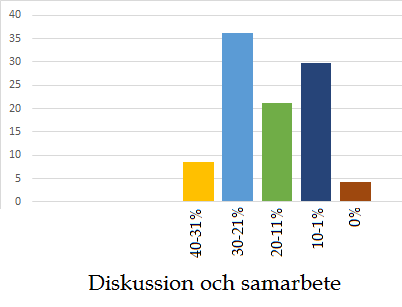
\includegraphics{Figures/Barcharts/diskussion.png}
    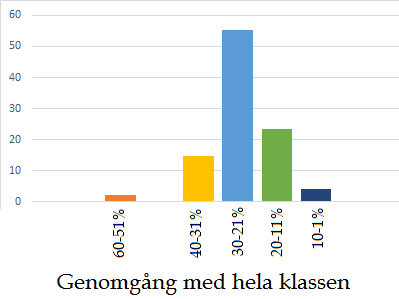
\includegraphics{Figures/Barcharts/genomgang.png}
    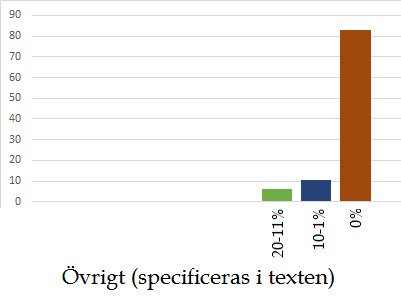
\includegraphics{Figures/Barcharts/ovrigt.png}
    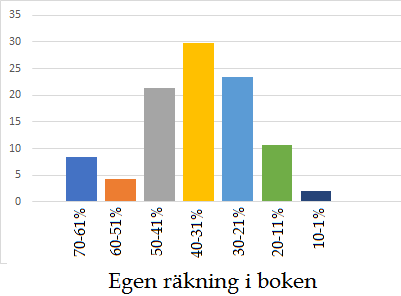
\includegraphics{Figures/Barcharts/rankning.png}
    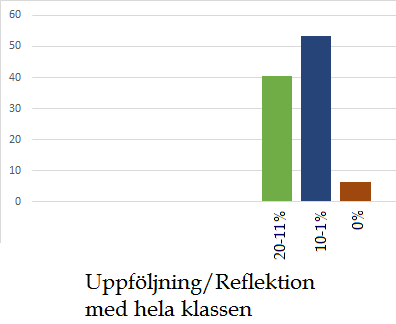
\includegraphics{Figures/Barcharts/uppfoljning.png}
    \caption{I figur (a)-(e) visas cirkeldiagram som visar hur stor andel av lektionstiden som olika lärare anger att de lägger på olika delar av undervisningen. Figur (f) visar det intervall (i procent) som varje färg representerar.}
    \label{fig:PC}
\end{figure}

\newpage

\textcolor{lila}{Genom att studera cirkeldiagrammen kan man notera att den största delen av lektionstiden används till genomgång och egen räkning. Därefter följer elevdiskussion och uppföljning, och utöver detta lägger en liten andel av lärarna även tid på andra saker. Under övrigt faller framförallt laborationer, spel, digitala quiz, redovisningar framförda av eleverna samt problemlösning.}

\textcolor{lila}{Några av lärarna kommenterade också i samband med den här frågan att de uppmuntrar eleverna att jobba tillsammans med uppgifterna i boken, och att det på så sätt blir mindre individuellt arbete, och mer diskussion mellan eleverna.}

\subsubsection{Vad är problemlösning för dig?}
\textcolor{lila}{Här bad vi lärarna att skriva en kort förklarande text om hur de definierar problemlösning. I de svar vi fick in kunde vi hitta några olika karatäriserande åsikter, och tittat på hur stor andel av lärarna som nämner de olika delarna.}

\textcolor{lila}{Många lyfte fram att ett problem är \textsl{en uppgift som man på förhand inte vet hur man ska lösa, och där man får applicera känd kunskap på nya situationer}. Detta är den vanligaste definitionen, och även den vi framförallt använder i denna rapport. Hela $79\%$ hade med detta som ett kriterium i sina definitioner av problemlösning.}

\textcolor{lila}{En annan viktig faktor, som nämndes av ungefär $20\%$, var \textsl{öppna problem}. Dessa definieras av att de går att lösa på flera olika sätt, och i vissa fall även kan ge olika svar. Ett exempel på ett öppet problem är att man ska planera en pool med en viss volym, vilket självklart kan göras på en mängd olika sätt.}

\textcolor{lila}{Därefter följde två kriterier, som vardera nämndes av cirka $16\%$. Det ena var att problemlösning \textsl{ska utgå från en större uppgift, vilken man måste använda flera olika metoder för att lösa}. Den andra pekar på att ett problem \textsl{innehåller för mycket eller för lite information}. Det innebär att man antingen måste sortera ut det man behöver eller finna ytterligare information, antingen genom att hitta denna via någon källa, eller genom egna uppskattningar.}

\textcolor{lila}{Ungefär $5\%$ av lärarna nämnde att \textsl{i par eller grupper} eftersom detta leder till \textsl{diskussion och reflektion} ($5\%$), att man använder sig av \textsl{modellering} ($5\%$) och att problemlösning handlar om att \textsl{tillämpa matematik} och därmed få en \textsl{verklighetsanknytning} ($5\%$). En liten andel poängterade att problemlösning ofta innebär att man \textsl{måste prova sig fram för att hitta en korrekt lösningsmetod}, och cirka $7\%$ tog upp att problemlösningsuppgifter ofta utgår från en \textsl{textuppgift}. En lärare svarade även enbart med ordet ''Textuppgifter''.}

\subsubsection{Mer problemlösning i matematiken}
\label{sec:MerProblemlosning}

\textcolor{lila}{Hela $91\%$ anger att de arbetar för att inkludera problemlösning i sin undervisning. Detta motiveras till viss del med att det ingår i kursplanen, vilket $19\%$ av lärarna nämner i sin motivering. Men utöver det skriver även hela $81\%$ av lärarna att de gör det för att det är viktigt med problemlösning. De poängterar att det är en stor del av matematiken, och att det är bra att kunna angripa problem man inte tidigare stött på i många sammanhang, och även inför framtiden. De $9\%$ som angav att de inte arbetade med problemlösning angav tidsbrist som en motverkande faktor. Det är mycket som behöver gås igenom, och då man ofta kan klara nationella provet utan problemlösning prioriteras detta ner. Någon sa också att det berodde på att de inte visste hur man skulle göra det på ett bra sätt, och att det är svårt att gå ifrån den undervisningsmetod man är van vid.}

\textcolor{lila}{När vi bad alla lärare att fundera på vad det finns för svårigheter med att införa mer problemlösning, fick vi många intressanta infallsvinklar. Av de som svarade nämnde $42\%$ att de tyckte att det är \textsl{svårt att hitta bra problem}. Ett bra problem ska ju vara utmanande för hela klassen, och då det ofta finns en mycket stor spridning i matematikkunskaperna hos en klass är detta inte helt lätt. Det tar också \textsl{tid}, och det nämns också som en stor bidragande faktor till varför man inte har mer problemlösning än man har, och nämns av $38\%$ av de svarande lärarna. Att elevernas tidigare skolår präglats till stor del av traditionell undervisning är också del av problematiken. $29\%$ av lärarna tar upp att eleverna ofta har för dåliga förkunskaper för att kunna ta sig an större problemuppgifter, samt att de också ofta är skeptiska till annan form av matematik än den de  är vana vid. Detta anges gälla speciellt för de högpresterande eleverna. En liten andel anger också att det som lärare kan vara svårt att ändra sin undervisning, och lätt att ''falla tillbaka i gamla hjulspår''.}

\textcolor{lila}{Trots dessa svårigheter är det ändå som sagt $91\%$ av lärarna som arbetar med att införa mer problemlösning i sin undervisning. Varför jobbar man så hårt med detta? Lärarna fick frågan om vad de ser för möjligheter med problemlösning. Många framhäver här att det är väldigt nyttigt att lära sig att tänka på nya sätt, och att även lyfta styrkorna i de olika tankesätten. Det är också viktigt att kunna hitta relevant information vid ett givet problem, och detta är färdigheter som kan appliceras i många fler sammanhang än bara vid skolbänken. Mer problemlösning nämns också som ett bra sätt att få tillämpa sin kunskap, och därmed få se hur matematikens många delar kan användas i verkligheten, vilket ger en relevans till ämnet. Det är också ett bra sätt för eleverna att träna på att samarbeta samt att få diskutera matematik, samt att det går att anpassa till olika nivåer. Rätt uppgift kan vara ett problem för en hel klass, och ger alla en chans att utgå från liknande villkor.}